\newpage

\section{Przegląd algorytmów i szczegóły implementacyjne}

Zaimplementowany w ramach platformy testowej proces rozpoznawania szczytów przebiega w podobny sposób, jak opisane w rozdziale \ref{section:teoretical_pipeline} podejście teoretyczne na podstawie analizy literaturowej. Na początku zbierane są dane z sensorów dotyczące kątów obrotu urządzenia oraz jego położenia GPS. Wykorzystując lokalizację określany jest współczynnik skalowania modelu związany ze zmianą wielkości pojedynczych kratek siatki terenu w zależności od szerokości geograficznej. Następnie generowany jest trójwymiarowy model ziemi z wykorzystaniem biblioteki OpenGL, a kamera ustawiana jest zgodnie z zebranymi danymi z czujników. Dla takiej wizualizacji określane są widoczne na niej szczyty górskie filtrując listę gór pochodzącą ze zbioru danych GeoNames. Zarówno dla wygenerowanej panoramy, jaki i wykonanego za pomocą aparatu urządzenia zdjęcia, wykrywane są krawędzie gór tworząc dwa obrazy binarne. Następnie wykorzystując metody dopasowania i sprawdzania podobieństwa między obrazami oraz listę widocznych wierzchołków na trójwymiarowym modelu stwierdzana zostaje ich widoczność na zdjęciu rzeczywistym. Odbywa się to~na~wygenerowanych obrazach binarnych, z których pobiera się odpowiedni wycinek w~zależności od~badanego szczytu. Dla tych gór, dla których stwierdzone zostanie podobieństwo z~odpowiednio dużym prawdopodobieństwem poprawności nakładane są etykiety nazw na~zdjęcie wejściowe. Tak zmodyfikowany obraz zostaje wysłany na wyjście procesu, a finalnie wyświetlony użytkownikowi. W przypadku działania na urządzeniu mobilnym w czasie rzeczywistym cykl ten powtarzany jest dla każdej kolejnej klatki nagrania zarejestrowanego na żywo. Diagram przedstawiający ten proces przedstawiono na rysunku \ref{fig:practical-pipeline}. Względem diagramu teoretycznego rozszerzony został on o dane pochodzące z sensorów oraz wykorzystanie aparatu urządzenia do pobrania kolejnych klatek obrazu.

\vspace{3em}

\begin{figure}[!h]
    \centering \includegraphics[width=1.0\linewidth]{img/flowchart_cale.drawio.png}
    \caption{Przepływ danych i sterowania procesu identyfikacji szczytów górskich z uwzględnieniem sensorów i urządzeń.}
    \label{fig:practical-pipeline}
\end{figure}


\subsection{Generowanie trójwymiarowego modelu terenu} \label{sec:szczegoly_generowanie_modelu}

Dane SRTM zapisane są w plikach jako ciąg wartości posortowanych zachód-wschód oraz północ-południe, które w ramach implementacji platformy testowej konwertowane są do postaci tablicy dwuwymiarowej. Numery rzędów i kolumn odpowiadają kolejno szerokości i długości geograficznej danego punktu, a wartości w poszczególnych komórkach tabeli to wysokość nad poziomem morza w danym miejscu. Takie przeskalowane ,,trójki'' (rząd, kolumna, wartość) odpowiadają współrzędnym trójwymiarowym OpenGL, a~w praktyce tworzą poszczególne wierzchołki modelu. W OpenGL prymitywy tworzy się z~siatki trójkątów i w ten sam sposób generowana jest mapa terenu w projekcie - trójkąty zostają utworzone z~kolejnych trzech posortowanych wierzchołków. Wizualizacja takiej siatki dla danych SRTM pokazana jest na rysunku \ref{fig:siatka}. Numerowane punkty odpowiadają kolejnym wartościom zapisanym w~tym zbiorze. 


\begin{figure}[!h]
    \centering \includegraphics[width=0.5\linewidth]{img/siatka.png}
    \caption{Wizualizacja tworzenia siatki trójkątów między punktami ze zbioru SRTM.}
    \label{fig:siatka}
\end{figure}

Dla tak stworzonych prymitywów dodawane jest cieniowanie zależne od położenia światła oraz wysokości poszczególnych punktów. Wymaga to obliczenia wektorów normalnych dla każdego wierzchołka. Uzyskuje się to poprzez normalizację sumy takich wektorów wszystkich trójkątów, w których skład wchodzi dany wierzchołek (wierzchołek częściowo opisuje od dwóch do sześciu trójkątów). Dzięki temu możemy w łatwy sposób kolorować i cieniować teren, co ma wpływ na detekcję krawędzi w dalszej części projektu, a także na poprawę walorów wizualnych przy ewentualnym podglądzie modelu.

Przykładowa wizualizacja trójwymiarowego terenu pokazano na rysunku \ref{fig:rendered}. Przedstawia ona wygenerowany model z ustawieniami lokalizacji i kątów obrotu odpowiadającym perspektywie zdjęcia \ref{fig:example-static-terrain-photo}. 

\begin{figure}[!h]
    \centering \includegraphics[width=0.45\linewidth]{img/rendered_scene.png}
    \caption{Przykład wizualizacji terenu z wykorzystaniem interfejsu OpenGL i danych SRTM.}
    \label{fig:rendered}
\end{figure}


\subsection{Widoczność szczytów górskich na trójwymiarowym modelu terenu} \label{sec:widocznosc_model}

Na model trójwymiarowy nanoszone są dane dotyczące szczytów górskich uzyskane ze~zbioru danych GeoNames. Zawierają one szerokość i długość geograficzną oraz wysokość nad poziomem morza dla każdego szczytu, które są przeliczane na odpowiadające położenie w~przestrzeni wygenerowanego terenu. Następnie, uzyskane w ten sposób wartości mapowane są na konkretny wierzchołek modelu. Tak przygotowane dane tworzą listę potencjalnie widocznych na zdjęciu wejściowym szczytów górskich. Ze względu jednak na to, że niektóre z~nich nie są widoczne na wizualizacji z perspektywy obserwatora musi zostać ona przefiltrowana.

Z tego powodu, na podstawie znajomości zagadnienia grafiki trójwymiarowej przez autora, został zaproponowany prosty, dwuetapowy proces filtracji listy potencjalnie widocznych wierzchołków. Oba kroki bazują na przystosowanych na potrzeby projektu metodach optymalizacji procesu renderingu poprzez usuwanie powierzchni niewidocznych. Jeśli potraktujemy szczyty górskie jako prymitywy i obiekty w generowanej scenie, to wykorzystanie takich algorytmów do określania ich widoczności wydaje się w pełni logiczne i uzasadnione. W~pierwszym etapie sprawdzane jest położenie poszczególnych punktów względem przestrzeni widzenia kamery. Następnie weryfikowana jest widoczność danego wierzchołka w kontekście bycia zasłanianym przez inne elementy terenu. Po przejściu tego procesu stwierdzana jest widoczność poszczególnych szczytów na wygenerowanym modelu.

\subsubsection{Filtracja szczytów poza polem widzenia kamery} \label{sec:frustum}

Pierwszym etapem filtrowania szczytów jest \textit{Frustum Culling} \cite{frutsum_culling}. Algorytm ten jest jedną z najpopularniejszych metod wykorzystywanych w grafice trójwymiarowej, której celem jest określenie wierzchołków znajdujących się w polu widzenia kamery. Dzięki temu pozwala usunąć obiekty, które nie znajdują się w zasięgu wzroku obserwatora. Polega on na projekcji współrzędnych trójwymiarowych na płaszczyznę dwuwymiarową obrazu. Na podstawie położenia kamery, kątów widzenia, kierunku patrzenia oraz innych, specyficznych dla danego rodzaju projekcji atrybutach tworzona jest matryca \textit{MVP} (z ang. Model View Projection \cite{MVP_matrices}). Opisuje ona przestrzeń widoczną dla kamery, a wizualnie charakteryzuje ostrosłup lub stożek ścięty. Przykładową wizualizację bryły widoczności dla projekcji perspektywicznej pokazano na rys. \ref{fig:frutsum-test}. Widoczne na niej obiekty w zacienionej przestrzeni - zielone koło - są odwzorowywane na obrazie, natomiast reszta jest usuwana - czerwone koła. Jeśli dany wierzchołek po przekształceniach z wykorzystaniem macierzy MVP ma prawidłowe współrzędne dwuwymiarowe - znajdujące się w zakresie szerokości i~wysokości tworzonego obrazu - to jest on widoczny dla obserwatora. 

\begin{figure}[!h]
    \centering \includegraphics[width=0.95\linewidth]{img/frutsum_test.png}
    \caption{Wizualizacja frustum culling. Ilustracja stożka widoczności kamery przy projekcji perspektywicznej. Odwzorowane zostaną tylko obiekty znajdujące się w przestrzeni stożka ściętego - zacieniona część. Czerwone koła będące poza obszarem widzenia kamery zostaną odrzucone. }
    \label{fig:frutsum-test}
\end{figure}


\par

Technika ta jest powszechnie stosowana w renderingu trójwymiarowym do optymalizacji tego procesu, ponieważ pozwala zmniejszyć liczbę wierzchołków oraz obiektów, które muszą być przetworzone i narysowane w generowanej scenie.

Na potrzeby pracy dyplomowej algorytm frustum culling został zaadaptowany do celów filtracji szczytów górskich, które na pewno nie są widoczne z perspektywy obserwatora, niezależnie od wygenerowanego terenu. Pozwala to znacznie zredukować listę potencjalnie widocznych szczytów na obrazie. 


\subsubsection{Filtracja zasłanianych szczytów} \label{sec:occlusion}

Dla pozostałych szczytów, które znajdują się w przestrzeni widocznej dla kamery, przeprowadzany jest tzw. \textit{Occlusion Culling} \cite{occlusion_culling}. Jest to kolejna technika optymalizacji procesu renderingu trójwymiarowego, której celem również jest odrzucenie struktur, które nie są widoczne z pozycji obserwatora. W tym wypadku znajdują się one jednak w~stożku widoczności ale położone są za innymi obiektami, więc są przez nie przesłaniane. Powoduje to, że nie muszą być przetwarzane i rysowane. Najprostsza implementacja wykorzystuje \textit{test głębokości} charakteryzujący to, jak blisko kamery znajduje się dany punkt, a co za tym idzie czy zasłania inne piksele (takie, które uzyskują mniejszą wartość współczynnika głębokości). 

\begin{figure}[!h]
    \centering \includegraphics[width=0.80\linewidth]{img/occlusion_culling.png}
    \caption{Wizualizacja Occlusion Culling. Czerwone koło jest przesłaniane przez zielony prostokąt, więc zostaje usunięte z procesu renderingu.}
    \label{fig:occlusion-culling}
\end{figure}

\par

W ramach opracowywanego procesu identyfikacji gór na obrazie occlusion culling pozwala sprawdzić, które wierzchołki odpowiadające poszczególnym szczytom przechodzą test głębokości. Jeśli dana góra uzyska dodatni wynik takiej próby to jest ona widoczna i powinna zostać oznaczona na obrazie. Test ten przeprowadzany jest z wykorzystaniem bufora zapytań (ang. queries \cite{queries_opengl}) w OpenGL. Taki mechanizm pozwala sprawdzać wynik wykonania danego zapytania. W projekcie sprawdzany jest stan wierzchołków (\textit{GL\_SAMPLES\_PASSED}) po przeprowadzeniu testu głębokości. Dla każdego szczytu wykonywana jest kwerenda i zależnie od odpowiedzi może on zostać usunięty z~listy potencjalnych szczytów górskich.

\par

Uzyskana po tym etapie lista zawiera szczyty, które na pewno są widoczne z perspektywy obserwatora na wygenerowanym trójwymiarowym modelu terenu. Następnym elementem jest dopasowanie ich do widocznych na zdjęciu wejściowym gór.


\subsubsection{Przykładowy rezultat widoczności szczytów górskich na wygenerowanym modelu}

Na rysunku \ref{fig:render_annotated} przedstawiono wcześniej wygenerowany model terenu (rys. \ref{fig:rendered}) z~naniesionymi nazwami widocznych na nim szczytów górskich. Ich widoczność została stwierdzona przy wykorzystaniu wyżej opisanego procesu filtrowania listy potencjalnie widocznych gór. Ze względu na duże zagęszczenie szczytów w widocznym na modelu paśmie górskim, liczba wyświetlanych nazw została ograniczona celem poprawy czytelności.  Dodatkowo obraz został wykadrowany z powodu zajmowania dużej części obrazu przez niebo oraz nieistotne elementy terenu.

\begin{figure}[!h]
    \centering \includegraphics[width=0.75\linewidth]{img/render_annotated.png}
    \caption{Przykładowy rezultat identyfikacji szczytów górskich na trójwymiarowym modelu terenu.}
    \label{fig:render_annotated}
\end{figure}


\subsection{Wyznaczanie odległości między dwoma punktami geograficznymi}

Jednym z obliczeń wykonywanych w trakcie procesu identyfikacji szczytów górskich wykonywanego na platformie testowej jest wyznaczanie odległości między dwoma punktami geograficznymi. Wyniki takich działań wykorzystywane są do ustalania odpowiedniej skali modelu trójwymiarowego względem rzeczywistości, ale również do wyliczenia odległości między obserwatorem, a widocznymi szczytami. Dlatego istotne było wybranie odpowiedniego algorytmu, który przy małej złożoności obliczeniowej będzie osiągać niski błąd. Przybliżone w następnym podrozdziale algorytmy były testowane w dalszej części pracy dyplomowej.

\subsubsection{Przegląd wybranych algorytmów}

W literaturze dostępnych jest wiele metod służących do obliczenia odległości między dwoma położeniami geograficznymi. Niektóre z nich wykorzystują elementy przybliżenia lub traktują kule ziemską jako inne figury trójwymiarowe, np. sferę lub walec. Na potrzeby pracy dyplomowej przybliżone zostały cztery algorytmy: sferyczne prawo cosinusów, metoda Haversiana, przybliżenie walcowe i iteracyjny algorytm Vincenta.

We wzorach poniżej występują następujące oznaczenia:

\begin{itemize}
    \item \textbf{d} - odległość między dwoma punktami geograficznymi.
    \item \textbf{R} - promień ziemi. Ze względu na różnicę pomiędzy promieniem równikowym i~biegunowym w projekcie wykorzystywany jest średni promień ziemi o długości $R=6371,0$~km \cite{promien_ziemi}.
    \item  \textbf{lat\textsubscript{i}} - (ang. latitude) szerokość geograficzna punktu \textit{i}
    \item  \textbf{long\textsubscript{i}} - (ang. longitude) wysokość geograficzna punktu \textit{i}
\end{itemize}



\paragraph{Sferyczne Prawo Cosinusów.} Jednym z podstawowych praw trygonometrii sferycznej jest \textit{Sferyczne Prawo Cosinusów} (ang. Spherical Law of Cosines). \cite{distance_geo} Jest to odpowiednik Prawa Cosinusów z geometrii płaskiej. Wykorzystywane jest do obliczania odległości między dwoma punktami na powierzchni sfery. Przy pomocy tej metody można uzyskać wynik charakteryzujący się dużą dokładnością, nawet przy małych odległościach.

\begin{align*}
    d=R * \arccos{(\sin{lat_{1}} * \sin{lat_{2}} + \cos{lat_{1}} * \cos{lat_{2}} * \cos{(long_{2} - long_{1}}))}
\end{align*}


\paragraph{Haversian.} Metoda \textit{Haversian} \cite{haversine,distance_geo} jest jedną z najczęściej wybieranych przy projektowaniu aplikacji wykorzystujących GPS czy bazujących na modelu ziemi. Została oparta na trygonometrii sferycznej jako jej uogólnienie. Pierwsze tabele haversianów były opisywane już na początku $XIX$ wieku, ale termin ten został sprecyzowany i opisany dopiero przez James'a Inmana w $1835$ roku.

\begin{align*}
    d=R * 2,0 * atan2(\sqrt{a}, \sqrt{1,0 - a})
\end{align*}
gdzie $a$ dane jest wzorem:
\begin{align*} \label{eq:formula}
\begin{gathered}
a = \sin{((lat_{2} - lat_{1})/2,0)}^{2} \\
    + \cos{lat_{1}} * \cos{lat_{2}} * \sin{((lat_{2} - lat{1}) / 2,0)}* \sin{((long_{2} - long_{1})/2,0)} 
\end{gathered}
\end{align*}

\paragraph{Przybliżenie walcowe równoodległościowe.} Następną z zaprezentowanych metod jest \textit{Przybliżenie Walcowe Równoodległościowe} (ang. Equirectangular Approximation). \cite{distance_geo} Algorytm ten opiera się na uproszczeniu, że Ziemia jest idealną sferą i traktuje ją jako płaszczyznę walcową. Sprawia to, że punkty o równej odległości względem równika na kuli ziemskiej są również tak samo odległe od równika na mapie. Dzięki takim założeniom zmniejszona zostaje złożoność obliczeniowa. Z tego powodu metoda ta jest często stosowana przy ograniczonych zasobach sprzętowych, na przykład w systemach wbudowanych.

\begin{align*}
d=R * \sqrt{((long_{2} - long_{1})*\cos{((lat_{1} + lat_{2})/2,0)})^{2} + (lat_{2}-lat_{1})^{2}}
\end{align*} 

\paragraph{Algorytm Vincenta.}
Ostatnim z opisywanych podejść jest iteracyjny algorytm Vincent'a. Jest to jedna z najbardziej zaawansowanych metod obliczania odległości geograficznej dająca bardzo dokładne rezultaty. Wadą tego rozwiązania jest duża złożoność, zarówno obliczeniowa jak i w kontekście opisu teoretycznego. Z tego powodu nie jest ona w pełni przybliżana w tej pracy dyplomowej. Dogłębnie opisana została w opracowaniu \cite{Vincenty}.



\subsection{Detekcja krawędzi gór} \label{sec:edge_detection}

Kolejnym etapem jest detekcja krawędzi na wygenerowanej panoramie oraz na rzeczywistym zdjęciu. Jest to istotny element procesu ze względu na to, że wyniki dla obu obrazów są do siebie porównywane, a następnie stwierdzana jest widoczność na nich poszczególnych szczytów.

\subsubsection{Oczekiwany rezultat} \label{sec:edge_detection_expected}

Wstępnie w ramach przeprowadzonych badań planowano wykrywać wszelkie krawędzie gór. Przykładowy oczekiwany rezultat zaprezentowano na rysunku \ref{fig:edge_detected_expected}. Jednak opracowanie odpowiedniej metody lub dobranie parametrów znanych algorytmów, tak by osiągnąć założony na początku cel okazało się niemożliwe w racjonalnej perspektywie czasu w kontekście tworzenie pracy dyplomowej magisterskiej, której tylko jednym z~elementów jest rozpoznawanie konturów. Głównym problemem było znalezienie uniwersalnego rozwiązania pozwalającego wykrywać w ten sposób krawędzie niezależnie od warunków pogodowych, jakości zdjęć czy innych zakłóceń.

\begin{figure}[!h]
    \centering \includegraphics[width=0.75\linewidth]{img/image-2023-03-04_072211_edge_expected_2.png}
    \caption{Przykład wstępnie oczekiwanego rezultatu detekcji krawędzi gór.}
    \label{fig:edge_detected_expected}
\end{figure}

Z tego względu zdecydowano się na ograniczenie detekcji krawędzi do najwyższych gór tworzących linię nieba. Jest to podejście podobne do opisanego w \cite{large-scale-visual}. Przykład wykrytych w ten sposób konturów pokazano na rysunku \ref{fig:edge_detected}. Konsekwencją takiego uproszczenia jest analiza jedynie szczytów górskich znajdujących się na tej linii oraz w bliskim jej sąsiedztwie ze względu na okno analizy o~pewnym rozmiarze. 



\begin{figure}[!h]
    \centering \includegraphics[width=0.75\linewidth]{img/image-2023-03-04_072211_edge.png}
    \caption{Przykład uproszczonej detekcji krawędzi gór.}
    \label{fig:edge_detected}
\end{figure}


Ma to szczególne znaczenie przy zdjęciach gór robionych z bliskiej odległości, gdy zajmują one dużą część obrazu w pionie oraz zawierają widoczne pasma górskie zróżnicowane pod względem wysokości. W takim przypadku efektem będzie pominięcie analizy wierzchołków znajdujących się w dolnej części zdjęcia, co finalnie oznacza niemożność ich identyfikacji. 

\subsubsection{Algorytm Canny} \label{sec:canny}

W ramach badań oraz platformy testowej, do celów detekcji krawędzi, zdecydowano się wybrać algorytm Canny \cite{Canny,SegmentationEdgeDetection,Canny_Opencv}. Mimo, że została opracowana w 1986 roku to dalej jest szeroko stosowaną metodą w przetwarzaniu cyfrowym obrazu rozwiązującą problem rozpoznawania konturów czy zmian w intensywności pikseli. Składa się ona z~czterech głównych etapów:

\begin{enumerate}
    \item \textbf{Usunięcie szumów.} Odbywa się to poprzez wygładzenie obrazu z wykorzystaniem filtru Gaussowskiego \cite{GaussianBlur} o rozmiarze jądra $5\textrm{x}5$. Pozwala to usunąć szum w postaci pojedynczych wyróżniających się pikseli. Efektem ubocznym jest bardziej rozmyte zdjęcie. 
    \item \textbf{Obliczenie siły i kierunek gradientu pikseli.} Na wygładzonym obrazie zastosowany zostaje operator Sobela \cite{Sobel} w pionie i poziomie celem określenia pierwszej pochodnej w obu tych kierunkach. Operator ten opiera się na splocie z macierzą $3\textrm{x}3$ wypełnioną wartościami zależnymi od orientacji. Następnie dla tych wyników oblicza się gradient oraz jego kierunek.
    \item \textbf{Tłumienie nie-maksymalne.} (ang. Non-maximum Suppression) \cite{Non-maximumSuppression} Polega na badaniu lokalnych maksimów dla znalezionych krawędzi. Dla piksela tworzącego dany kontur porównuje się go z wynikiem sąsiadów wzdłuż gradientu. Jeśli dany punkt jest lokalnym maksimum to uznawany jest za składową krawędzi. W innym przypadku jest odrzucany. Pozwala zachować piksele z najbardziej widoczną zmianą intensywności w danym otoczeniu.
    \item \textbf{Progowanie Histerezowe.} (ang. Hysteresis Thresholding) \cite{LectureComputerVision} Jest to filtrowanie krawędzi w zależności od siły gradientu. Opiera się na dwóch progach. Jeśli piksel znajduje się powyżej tych wartości to jest on uznawany za pewną (mocną) krawędź, natomiast jeśli poniżej to jest odrzucany. Piksele, których wartość gradientu znajduje się między progami zostają uznane za kontur w zależności od tego czy są połączone z~jakąś mocną krawędzią, czy nie.
\end{enumerate}

\vspace{5mm}

Parametry progowania histerezowego w implementacji platformy testowej zostały ustawione w taki sposób, żeby odrzucać głównie zaszumienie w części zdjęcia zawierającej niebo. Związane jest to z wcześniej opisanym problemem i decyzją o analizie jedynie najwyższych gór. Dla wynikowego obrazu binarnego wyszukuje się najwyższe krawędzie odrzucając te znajdujące się poniżej. Dlatego szum i dodatkowe wskazania w niższej części obrazu nie mają tak wielkiego znaczenia jak te na niebie, ponieważ nie są brane w~ogóle pod uwagę w trakcie analizy. Uzyskany efekt zawiera pojedynczy kontur w danej kolumnie zdjęcia tak jak na rysunku \ref{fig:edge_detected}. Taki sam schemat detekcji krawędzi stosowany jest w przypadku panoramy trójwymiarowego modelu terenu. W tym przypadku dobranie parametrów było dużo prostsze ze względu na stałe odwzorowanie kolorów takiego modelu. 

\subsection{Dopasowanie obrazów binarnych} \label{sec:dopasowanie}

Pomijając dodawanie nazw widocznych szczytów na zdjęciu rzeczywistym, dopasowanie obrazów binarnych celem stwierdzenia widoczności owych gór jest ostatnim etapem opracowywanego procesu ich identyfikacji. Wydaje się on również najważniejszym w~kontekście całego projektu, ponieważ to wyniki porównania ze sobą obrazów wygenerowanego modelu oraz faktycznego zdjęcia gór wpływają na odrzucenie lub etykietowane poszczególnych szczytów. Jeśli dany algorytm nie będzie w stanie dopasować do siebie badanych zdjęć z odpowiednio wysoką pewnością, szczyt może być niesłusznie uznany za niewidoczny, lub odwrotnie, niewidoczny szczyt jako widoczny. Z tego powodu, analiza tego zagadnienia oraz dostępnych algorytmów była bardziej dogłębna, a metody lepiej przetestowane.  



Operacja dopasowania obrazów zawierających krawędzie gór odbywa się na ich wycinkach o pewnym rozmiarze. W przypadku obrazu binarnego wyrenderowanego modelu centralnym punktem takiego fragmentu był piksel odpowiadający wierzchołkowi danego szczytu. Natomiast, dla zdjęcia wejściowego centrum było estymowane jako takie samo jak wizualizacji. Można przyjąć, że jest to miejsce hipotetycznego szczytu, gdyby wskazania sensorów urządzenia były idealne. Jednak ze względu, że w rzeczywistości takie mogą nie być, wycinek ten jest większy niż obrazu wygenerowanego terenu. Powiększony on jest o~pewną tolerancję, celem zwiększenia pewności zawierania się w nim widocznego szczytu. 

W poniższych podrozdziałach opisano dwie metody, które w ramach pracy dyplomowej były badane. Są to algorytmy oparte na dopasowaniu: wzorca (ang. template matching) oraz cech (ang. feature matching). Pierwsza z nich bada wartości pojedynczych pikseli, natomiast druga bierze pod uwagę kontekst poszczególnych punktów


\subsection{Dopasowanie na podstawie wzorca} \label{sec:template_matching}

Pierwszą z opisanych metod porównywania obrazów jest dopasowanie na podstawie wzorca (czasem określana także jako dopasowanie szablonu) \cite{template_opencv_1,template_opencv_2,template_adaptive,template_british,template_vidhya}. Do swojego działania wykorzystuje metody obliczania korelacji między dwoma zbiorami (w tym wypadku pikseli) dla każdego położenia. Dla danego położenia okna wynikiem takich obliczeń jest podobieństwo między dwoma obrazami. Finalnie, metoda ta zwraca najbardziej prawdopodobną lokalizację, w której szablon może znajdować się na zdjęciu wejściowym oraz jak pewne jest ich podobieństwo.

Ze względu na wykorzystanie jedynie numerycznych form porównania, metoda ta jest podatna na różne zniekształcenia między obrazami takie jak skalowanie czy rotacja, a~także na różnice w intensywności. Z tego względu może być efektywna przy porównywaniu prostych obrazów oraz przy kontrolowanych warunkach ich pozyskiwania. W kontekście porównywania obrazów binarnych zawierających kontury gór założenia te wydają się spełnione, co może przekładać się na lepsze wyniki \cite{feature_vs_template}.

Algorytmy oparte o analizę dopasowania wzorca tworzą tzw. mapę odpowiedzi lub mapę podobieństwa. Jest to dwuwymiarowa tablica o takich samych rozmiarach jak zdjęcie wejściowe, na którym szukany jest dany szablon. Wypełniania jest obliczonymi współczynnikami podobieństwa $R(x,y)$ dla każdego położenia wzorca względem głównego obrazu. Wykonywane jest to przesuwając szablonu po wszystkich pikselach obrazu wejściowego. Tak stworzona mapa zawiera w każdej komórce ustalony współczynnik dopasowania opisujący jak podobne są do siebie oba obrazy. Im wyższa jego wartość tym zdjęcia bardziej do siebie pasują. W przypadku wartości znormalizowanych pełną zgodność stwierdza się przy osiągnięciu wartości $1,0$ - obrazy są wtedy identyczne przy danym położeniu. Przykładowy wynik dopasowania wycinka wygenerowanego modelu trójwymiarowego do zdjęcia rzeczywistego w projekcie pokazany został na rysunku \ref{fig:template_matching_map}. Bardziej intensywny biały kolor na grafice oznacza wyższe wskaźnik podobieństwa między nimi (zakres wartości podobieństwa $0,0-1,0$ został przeskalowany na wartość pikseli $0-255$ w skali szarości). Na środku widoczny jest najbardziej jasny punkt - jest to najbardziej prawdopodobne położenie poszukiwanego szczytu. 


\begin{figure}[!h]
    \centering \includegraphics[width=0.6\linewidth]{img/template_matching_map.png}
    \caption{Przykład mapy podobieństwa uzyskanej wykorzystując algorytm dopasowania wzorca przy porównaniu obrazów binarnych krawędzi gór.}
    \label{fig:template_matching_map}
\end{figure}


W bibliotece OpenCV występują trzy metody obliczania wartości w mapie dopasowania: kwadrat różnicy (ang. Squared Difference - SQDIFF), korelacja krzyżowa (ang. Cross-correlation - CCORR), współczynik korelacji krzyżowej (ang. Cross-correlation coefficient - CCOEFF). Wszystkie z nich występują zarówno w wersji bez, jak i z normalizacją \cite{template_opencv_1}\cite{template_opencv_2} do zakresu wartości $0,0-1,0$. 

W trakcie prac badawczych wykorzystane zostały tylko metody oparte na korelacjach (CCORR i CCOEFF). Kwadrat różnicy został całkowicie pominięty z opisu teoretycznego oraz z porównań algorytmów z dalszej części pracy dyplomowej. Związane jest to z bardzo słabymi, bliskimi zeru, wynikami testów wstępnych. Dodatkowo, badania te pokazały przewagę wersji znormalizowanych korelacji krzyżowej i współczynnika korelacji, nad ich wersjami bez normalizacji. Związane to jest z łatwiejszym doborem parametrów przy ograniczonym zakresie wartości. Z tego powodu brane pod uwagę są tylko metody z~normalizacją. 

W opisanych poniżej równaniach stosowanych do wypełnienia mapy podobieństwa wykorzystywane są następujące oznaczenia:

\begin{itemize}
    \item $\textbf{R(x, y)}$ - wyliczony współczynnik podobieństwa wzorca i zdjęcia wejściowego przy położeniu okna  o środku $x, y$. Całościowo $R$ oznacza tzw. mapę odpowiedzi/podobieństwa zawierającą obliczony współczynnik w każdej lokalizacji.
    \item $\textbf{x, y}$ - współrzędne danego piksela zdjęcia wejściowego.
    \item $\textbf{x',y'}$ - współrzędne danego piksela wzorca.
    \item $\textbf{I(x, y)}$ - wartość/intensywność/jasność piksela zdjęcia wejściowego o danych współrzędnych.
    \item $\textbf{T(x',y')}$ - wartość/intensywność/jasność piksela wzorca o danych współrzędnych.
\end{itemize}



\paragraph{Znormalizowana korelacja krzyżowa.}
Metoda ta wykorzystuje korelację krzyżową jako metrykę podobieństwa. Mierzy ona dopasowanie szablonu i zdjęcia wejściowego dla każdej możliwej pozycji drugiego obrazu. W praktyce polega ona na przesuwaniu okna analizy po całym obrazie wejściowym i dla każdej takiej lokalizacji obliczany jest iloczyn skalarny wartości pikseli. Wyższa wartość korelacji wskazuje na większe podobieństwo między szablonem, a obszarem docelowym.

Wersja ta skupia się wyłącznie na korelacji punktowej. Z tego powodu jest ona skuteczna głównie w przypadku, gdy dopasowane obrazy mają podobny zakres jasności oraz minimalne zniekształcenia względem siebie takie jak rotacja czy skalowanie.

Wartości w mapie dopasowania, dla tej metody, obliczane są zgodnie z równaniem:

\begin{align*}
    R(x,y)= \frac{\sum_{x',y'} (T(x',y') \cdot I(x+x',y+y'))}{\sqrt{\sum_{x',y'}T(x',y')^2 \cdot \sum_{x',y'} I(x+x',y+y')^2}}
\end{align*}



\paragraph{Znormalizowany współczynnik korelacji.}
Metoda ta również wykorzystuje korelację krzyżową oraz iloczyn skalarny wartości pikseli. Stosuje ona dodatkowo normalizację uśredniającą jasności obrazu do zera. Z tego powodu w przeciwieństwie do poprzedniego rozwiązania nie skupia się wyłącznie na korelacji punktowej, ale również bierze pod uwagę różnice w intensywności pikseli w danym otoczeniu. Dzięki temu, wersja ta jest bardziej elastyczna i odporniejsza na zmianę warunków oświetleniowych czy kontrastu między zdjęciami oraz na różnego typu zniekształcenia.  

Miara podobieństwa opisana jest wzorem:

\begin{align*}
    R(x,y)= \frac{ \sum_{x',y'} (T'(x',y') \cdot I'(x+x',y+y')) }{ \sqrt{\sum_{x',y'}T'(x',y')^2 \cdot \sum_{x',y'} I'(x+x',y+y')^2} }
\end{align*}

gdzie $T'$ i $I'$ dane są wzorami:

\begin{align*}
    \begin{array}{c}
        T'(x',y')=T(x',y') - 1/(w \cdot h) \cdot \sum _{x'',y''} T(x'',y'') \\ 
        I'(x+x',y+y')=I(x+x',y+y') - 1/(w \cdot h) \cdot \sum _{x'',y''} I(x+x'',y+y'') 
    \end{array}
\end{align*}

$T'$ i $I'$ oznaczają wartość danego piksela, odpowiednio dla szablonu i zdjęciu wejściowego, poddaną normalizacji uśredniającej względem jasności otoczenia. Sprawia ona, że wskazania średnie w danym punkcie przyjmują wartość $0$. Natomiast pozostałe wyniki równania określają odległość wartości jasności pikseli od średniej.



\subsection{Dopasowanie na podstawie cech} \label{sec:feature_matching}

Drugą metodą detekcji podobieństwa między obrazami wykorzystywaną w projekcie pracy dyplomowej jest dopasowanie na podstawie cech (z ang. Feature Matching). Polega ona na porównywaniu między zdjęciami pewnych, charakterystycznych cech - stąd nazwa metody. Mogą być nimi m.in.: krawędzie, tekstury, nieszablonowe zmiany jasności czy elementy wyróżniające się w danej przestrzeni. Na ich podstawie, wyszukując podobne struktury na obu zdjęciach, stwierdza się ich podobieństwo \cite{opencv_understand_features}\cite{feature_lieberman}. 

Metoda ta jest jedną z częściej wykorzystywanych w procesie tzw. rejestracji zdjęć (ang. Image Registration) lub inaczej nazywane wyrównaniem zdjęć (ang. Image Alignment) \cite{szelinski}. Są to techniki mające na celu zarejestrować i wyrównać obrazy zawierające tę samą scenę lub obiekt ale z różnych punktów widzenia czy w różnych warunkach oświetleniowych~\cite{image_reg_geeks,image_reg_pyimage}. Pozwalają one uzyskać dla nich jednolity układ współrzędnych, przeprowadzić korekcję zniekształceń, tworzyć z wielu zdjęć panoramę lub zdjęcia trójwymiarowe, a~także, co istotne w kontekście pracy dyplomowej, porównywać obrazy. Z~powodzeniem jednak rejestrowanie zdjęć wykorzystywane jest również w przetwarzaniu dokumentów czy śledzeniu obiektów na nagraniach \cite{image_reg_practical}. 

W teorii, feature matching jest bardziej elastyczny niż metoda oparta na szablonach oraz bardziej odporna na zniekształcenia, rotacje czy skalowanie. Daje ona dobre wyniki przy skomplikowanych scenach bogatych w unikalne cechy, ze zmiennymi widokami oraz przy poszukiwaniu złożonych struktur o nietrywialnych elementach. Jednocześnie radzi sobie gorzej z prostymi scenami, w szczególności podczas wyszukiwania konkretnego wzoru lub prymitywnych obiektów o ograniczonej możliwości transformacji. Z tego powodu może się okazać mało skuteczna przy porównywaniu obrazów binarnych krawędzi gór, które nie zawierają zbyt dużej liczby charakterystycznych cech, a jedynie zbiór białych linii na jednolitym tle.


Podejście to składa się z kilku etapów. Na początku wybierane są punkty charakterystyczne, zawierające pewnego rodzaju szczególne cechy. Określane są dla nich również deskryptory opisujące wybrane ich właściwości. Odbywa się to dla zdjęć wejściowych: poszukiwanego oraz przeszukiwanego. Następnie porównuje się punkty z obu obrazów, dopasowując do siebie te z największym podobieństwem. Ze względu na możliwe szumy i~błędne przyporządkowania, należy je odpowiednio przefiltrować i odrzucić niepoprawne. Ostatnim krokiem jest przekształcenie szablonu na podstawie dopasowanych punktów kluczowych, w taki sposób by poprawnie określić miejsce szukanego obiektu na drugim obrazie. 



\subsubsection{Punkty kluczowe i ich deskryptory} \label{sec:feature_matching_keypoints}

Pierwszym etapem dopasowania obrazów na podstawie cech jest wyszukanie punktów kluczowych oraz ich deskryptorów \cite{affine_point}\cite{feature_cornell}. Są one podstawą działania tego rodzaju algorytmów, ponieważ są ze sobą porównywane w celu stwierdzenia podobieństwa danych elementów zdjęć.

Punkty charakterystyczne określają specyficzne lub wyjątkowe obszary na zdjęciu, sklasyfikowane na podstawie wyróżnionych unikalnych cech. Z tego względu mogą być jednoznacznie identyfikowane w różnych widokach, a nawet na różnych zdjęciach. Ich obszary mogą być specyficzne ze względu na różne atrybuty, takie jak: wzór, tekstura, strukturę jaką tworzą lub poprzez krawędzie i kąty. Dany punkt by mógł zostać uznany za kluczowy musi spełniać określone niezmienniki, tzn. musi być niezależny od transformacji takich jak skalowanie, rotacja, zmiany jasności czy perspektywy. Kolejnym założeniem odnoszącym się do punktów kluczowych jest powtarzalność. Musi być możliwość identyfikacji tych samych cech na kolejnych scenach lub obrazach. Wizualizację wykrytych na obrazie binarnym punktów charakterystycznych wraz z ich kierunkiem oraz rozmiarem pokazano na rysunku \ref{fig:feature_keypoints}.

\begin{figure}[!h]
    \centering \includegraphics[width=0.6\linewidth]{img/keypoints.png}
    \caption{Przykład części wykrytych punktów charakterystycznych wraz z ich kierunkiem i~rozmiarem na obrazie binarnym krawędzi gór.}
    \label{fig:feature_keypoints}
\end{figure}


Cechy punktów kluczowych opisywane są przez tak zwane deskryptory tworzone dla każdego miejsca charakterystycznego. Zawierają głównie informację na temat otoczenia danego punktu. Opisują intensywność pikseli, kierunek ewentualnych gradientów, wzór, który tworzy czy jego histogram. Zestaw tych cech jest niezależny od lokalizacji, dzięki czemu pozostałe fragmenty obrazu nie mają na niego wpływu i może być porównywany między różnymi scenami. Deskryptory najczęściej przybierają formy wektorowe. 

\paragraph{SIFT.} Przykładem algorytmu pozwalającego na wyszukiwanie opisanych punktów i cech jest SIFT (z ang. Scale-Invariant Feautre Transform) \cite{SIFT}\cite{SIFT_opencv}. Składa się on z kilku etapów. Pierwszym jest poszukiwanie potencjalnych punktów kluczowych poprzez zastosowanie techniki \textit{Różnicy Gaussów} (ang. Difference of Gaussian). Jest to technika nakładania filtrów gaussa o dwóch rozmiarach okna, a następnie obliczaniu różnicy wartości pikseli między nimi. Celem tego jest wyszukanie punktów niezależnych od skalowania. Wyszukując ich ekstrema uzyskuje się wstępną listę punktów charakterystycznych o różnych rozmiarach. Kolejnym etapem jest ich filtracja ze względu na kontrast (niski kontrast może oznaczać wrażliwość na szum) lub odrzucając mniej istotne krawędzie. Wykonywane jest to na podstawie progowania o pewnym ustalonym progu dla lokalnych ekstremów. Pozostałe punkty charakterystyczne traktowane są jako stabilne i wartościowe. Następnie dla każdego z nich określany jest kierunek oraz rozmiar, w zależności od jego sąsiedztwa. Pozwala to uodpornić algorytm na zmiany rotacji względem kolejnych scen. Na końcu obliczane są deskryptory cech okolicy danego punktu.



\paragraph{ORB.} Drugą z opisywanych metod służących do określania punktów charakterystycznych oraz ich deskryptorów jest ORB (z ang. Oriented FAST and Rotated BRIEF) \cite{ORB}\cite{ORB_opencv}. Jest to połączenie algorytmów FAST (z ang. Features from Accelerated Segment Test \cite{fast}) do wykrywania punktów kluczowych oraz BRIEF (z ang. Binary Robust Independent Elementary Features \cite{brief}) do opisu cech. Ze względu na jej hipotetyczną wydajność autor artykułu, w którym opisuje tę metodę, zatytułował go \textit{ORB: Efektywna alternatywa dla SIFT oraz SURF} (oryg. \textit{ORB: An effective alternative to SURF and SIFT} \cite{ORB}). Nazwa ta związana jest z mniejszą złożonością obliczeniową, a co za tym idzie krótszym czasem wykonania. Odnosi się również do patentów, którymi były objęte oba algorytmy. W przeciwieństwie do nich, ORB od razu był wolny od takich ograniczeń (SIFT był opatentowany w momencie powstania tamtego artykułu, lecz licencja ta wygasła w marcu 2020 r.). Ze względu, że FAST nie był odporny na obroty scen, w algorytmie ORB obliczana jest orientacja punktów, opisywana w formie kołowej. Modyfikuje on również metodę BRIEF wykorzystując obliczoną wcześniej rotację. Tworzone są na ich podstawie macierze obrotu, służące do nadawania deskryptorom kierunku. Ma to na celu zniwelowanie problemów algorytmu BRIEF z wydajnością. Dzieje się to jednak kosztem utraty wysokiej wariancji oraz nieskorelowania punktów. By odzyskać te cechy ORB przeprowadza zachłanne przeszukiwanie potencjalnych wartości wynajdując takie, które posiadają te właściwości. 



\subsubsection{Dopasowanie punktów kluczowych obu zdjęć} \label{sec:feature_matching_matching}

Obliczone punkty charakterystyczne oraz ich deskryptory dla obu zdjęć należy ze sobą porównać i przyporządkować do siebie najbardziej pasujące tworząc pary. Wykonywane jest to poprzez zestawienie ze sobą poszczególnych cech z obu zdjęć. Popularnymi metodami porównywania punktów kluczowych oraz deskryptorów są na przykład: algorytm siłowy (ang. Brute Matching) lub FLANN (z ang. Fast Library for Approximate Nearest Neighbors) \cite{opencv_matching}\cite{feature_unik}.

Jak wszelkiego rodzaju algorytmy siłowe, tak i w tym przypadku polega on na przeszukiwaniu przestrzeni rozwiązania poprzez sprawdzenie wszystkich możliwych kombinacji i wybraniu najlepszych. Dany punkt charakterystyczny z dopasowywanego szablonu porównuje się z każdym punktem ze zdjęcia, na którym poszukujemy interesujący nas obiekt. Na podstawie takich porównań tworzy się pary o największym podobieństwie. Zaletą takiego rozwiązania jest gwarancja uzyskania rezultatów optymalnych z najlepszymi dopasowaniami. Wadą podejścia opartego na metodach siłowych jest natomiast długi czasu wykonania oraz wykorzystanie większych zasobów pamięciowych. Złożoność obliczeniowa tego algorytmu wynosi $O(n^2)$.

FLANN \cite{FLANN} \cite{FLANN_manual} zorientowany jest na szybkie znajdowanie najbliższych sąsiadów. W~praktyce nie jest to jedna metoda, a zbiór algorytmów służących do tego celu. W zależności od użytych parametrów takich jak sposób indeksowania, liczba epok, wymagana dokładność czy preferowana metoda możliwe jest uzyskanie różnych rezultatów. W cytowanej dokumentacji FLANN zasugerowane są optymalne ustawienia dla wybranych algorytmów wyszukujących punkty charakterystyczne, w tym dla opisanych w poprzednim podrozdziale ORB i SIFT. Zgodnie z założeniem mają być to szybkie rozwiązania, a~osiągane jest to kosztem znajdowania tylko przybliżonego rozwiązania. Z tego względu może on dawać mniej dokładne wyniki niż na przykład metoda siłowa. W tym przypadku, średnia złożoność obliczeniowa jest na poziomie $O(\log(n))$, co ma znaczenie przy dużych zbiorach danych. 

Przy obu podejściach, możliwe jest uzyskanie dla każdego punktu $k$ najbliższych sąsiadów (w przypadku metody siłowej $k$ najlepszych). Ze względu na liczbę punktów charakterystycznych oraz wartość ich dopasowania zasadnym staje się wybór tylko pewnej ich części w zależności od przyjętego kryterium. W projekcie magisterskim, jeśli dopasowywany jest tylko jeden punkt wykorzystywana jest filtracja za pomocą progowania podobieństwa. W przypadku $k\geq2$ wykorzystywany jest tzw. test współczynników. Określa on jak bardzo lepsze musi być pierwsze z $k$ dopasowań w porównaniu do pozostałych, by para mogła być uznana za wartościową. Jeśli przykładowo pierwszy i drugi mają porównywalną wartość podobieństwa to dopasowania dla tego punktu zostają odrzucone. 

Na rysunku \ref{fig:matched_points} przedstawiono przykład dopasowanych punktów kluczowych dla krawędzi gór wygenerowanego modelu oraz rzeczywistego zdjęcia. Do celów wizualizacyjnych zostało wybrane $10$ dopasowań o najwyższym współczynniku podobieństwa, celem zwiększenia przejrzystości.

\begin{figure}[!h]
    \centering \includegraphics[width=0.7\linewidth]{img/matched_points.png}
    \caption{Przykład dopasowanych punktów kluczowych dwóch obrazów binarnych krawędzi gór.}
    \label{fig:matched_points}
\end{figure}

\subsubsection{Projekcja położenia z wykorzystaniem homografii} \label{sec:feature_matching_homography}

Rozłożenie połączonych punktów może tworzyć nieregularne kształty. Z tego powodu dopasowanie szablonu na zdjęciu rzeczywistym z odpowiednią skalą, rotacją i zniekształceniami jedynie na podstawie tych połączeń może być wizualnie trudnym zadaniem. Do tego celu może być wykorzystana estymacja z wykorzystaniem transformacji homograficznej \cite{homography_aids}. 

Homografia opisuje relacje płaską między dwoma obrazami z różnych punktów obserwacji. Reprezentowana jest poprzez macierz $3\textrm{x}3$ z ośmioma punktami swobody, tworzącą tak zwaną macierz transformacji perspektywicznej. Ten rodzaj przekształcenia zachowuje proste, czteropunktowe kontury obrazu, ale pozwala na deformacje obrazu bez zachowania sztywności elementów. Przy jej użyciu możliwa jest projekcja pikseli na wybraną płaszczyznę \cite{homography_opencv_explain}\cite{homography_maulion}.


W kontekście porównania obrazów na podstawie cech technika ta pozwala na transformację szablonu względem dopasowanych punktów kluczowych. Wykonywane jest to w~taki sposób, że możliwe jest jego nałożenie na obraz główny z jak najlepszym wyrównaniem i odwzorowaniem przekształceń. Pozwala to również na stwierdzenie dokładnego położenia szukanego fragmentu obrazu \cite{homography_opencv}. Przykład takiej transformacji z zaznaczeniem pewnej liczby punktów kluczowych oraz oznaczeniem szukanego obiektu pokazany został na rysunku \ref{fig:homography} (ze względu na małą przejrzystość takiej grafiki przy dopasowaniu krawędzi gór, do celów prezentacyjnych wykorzystany został prosty obiekt świata rzeczywistego). 


\begin{figure}[!h]
    \centering 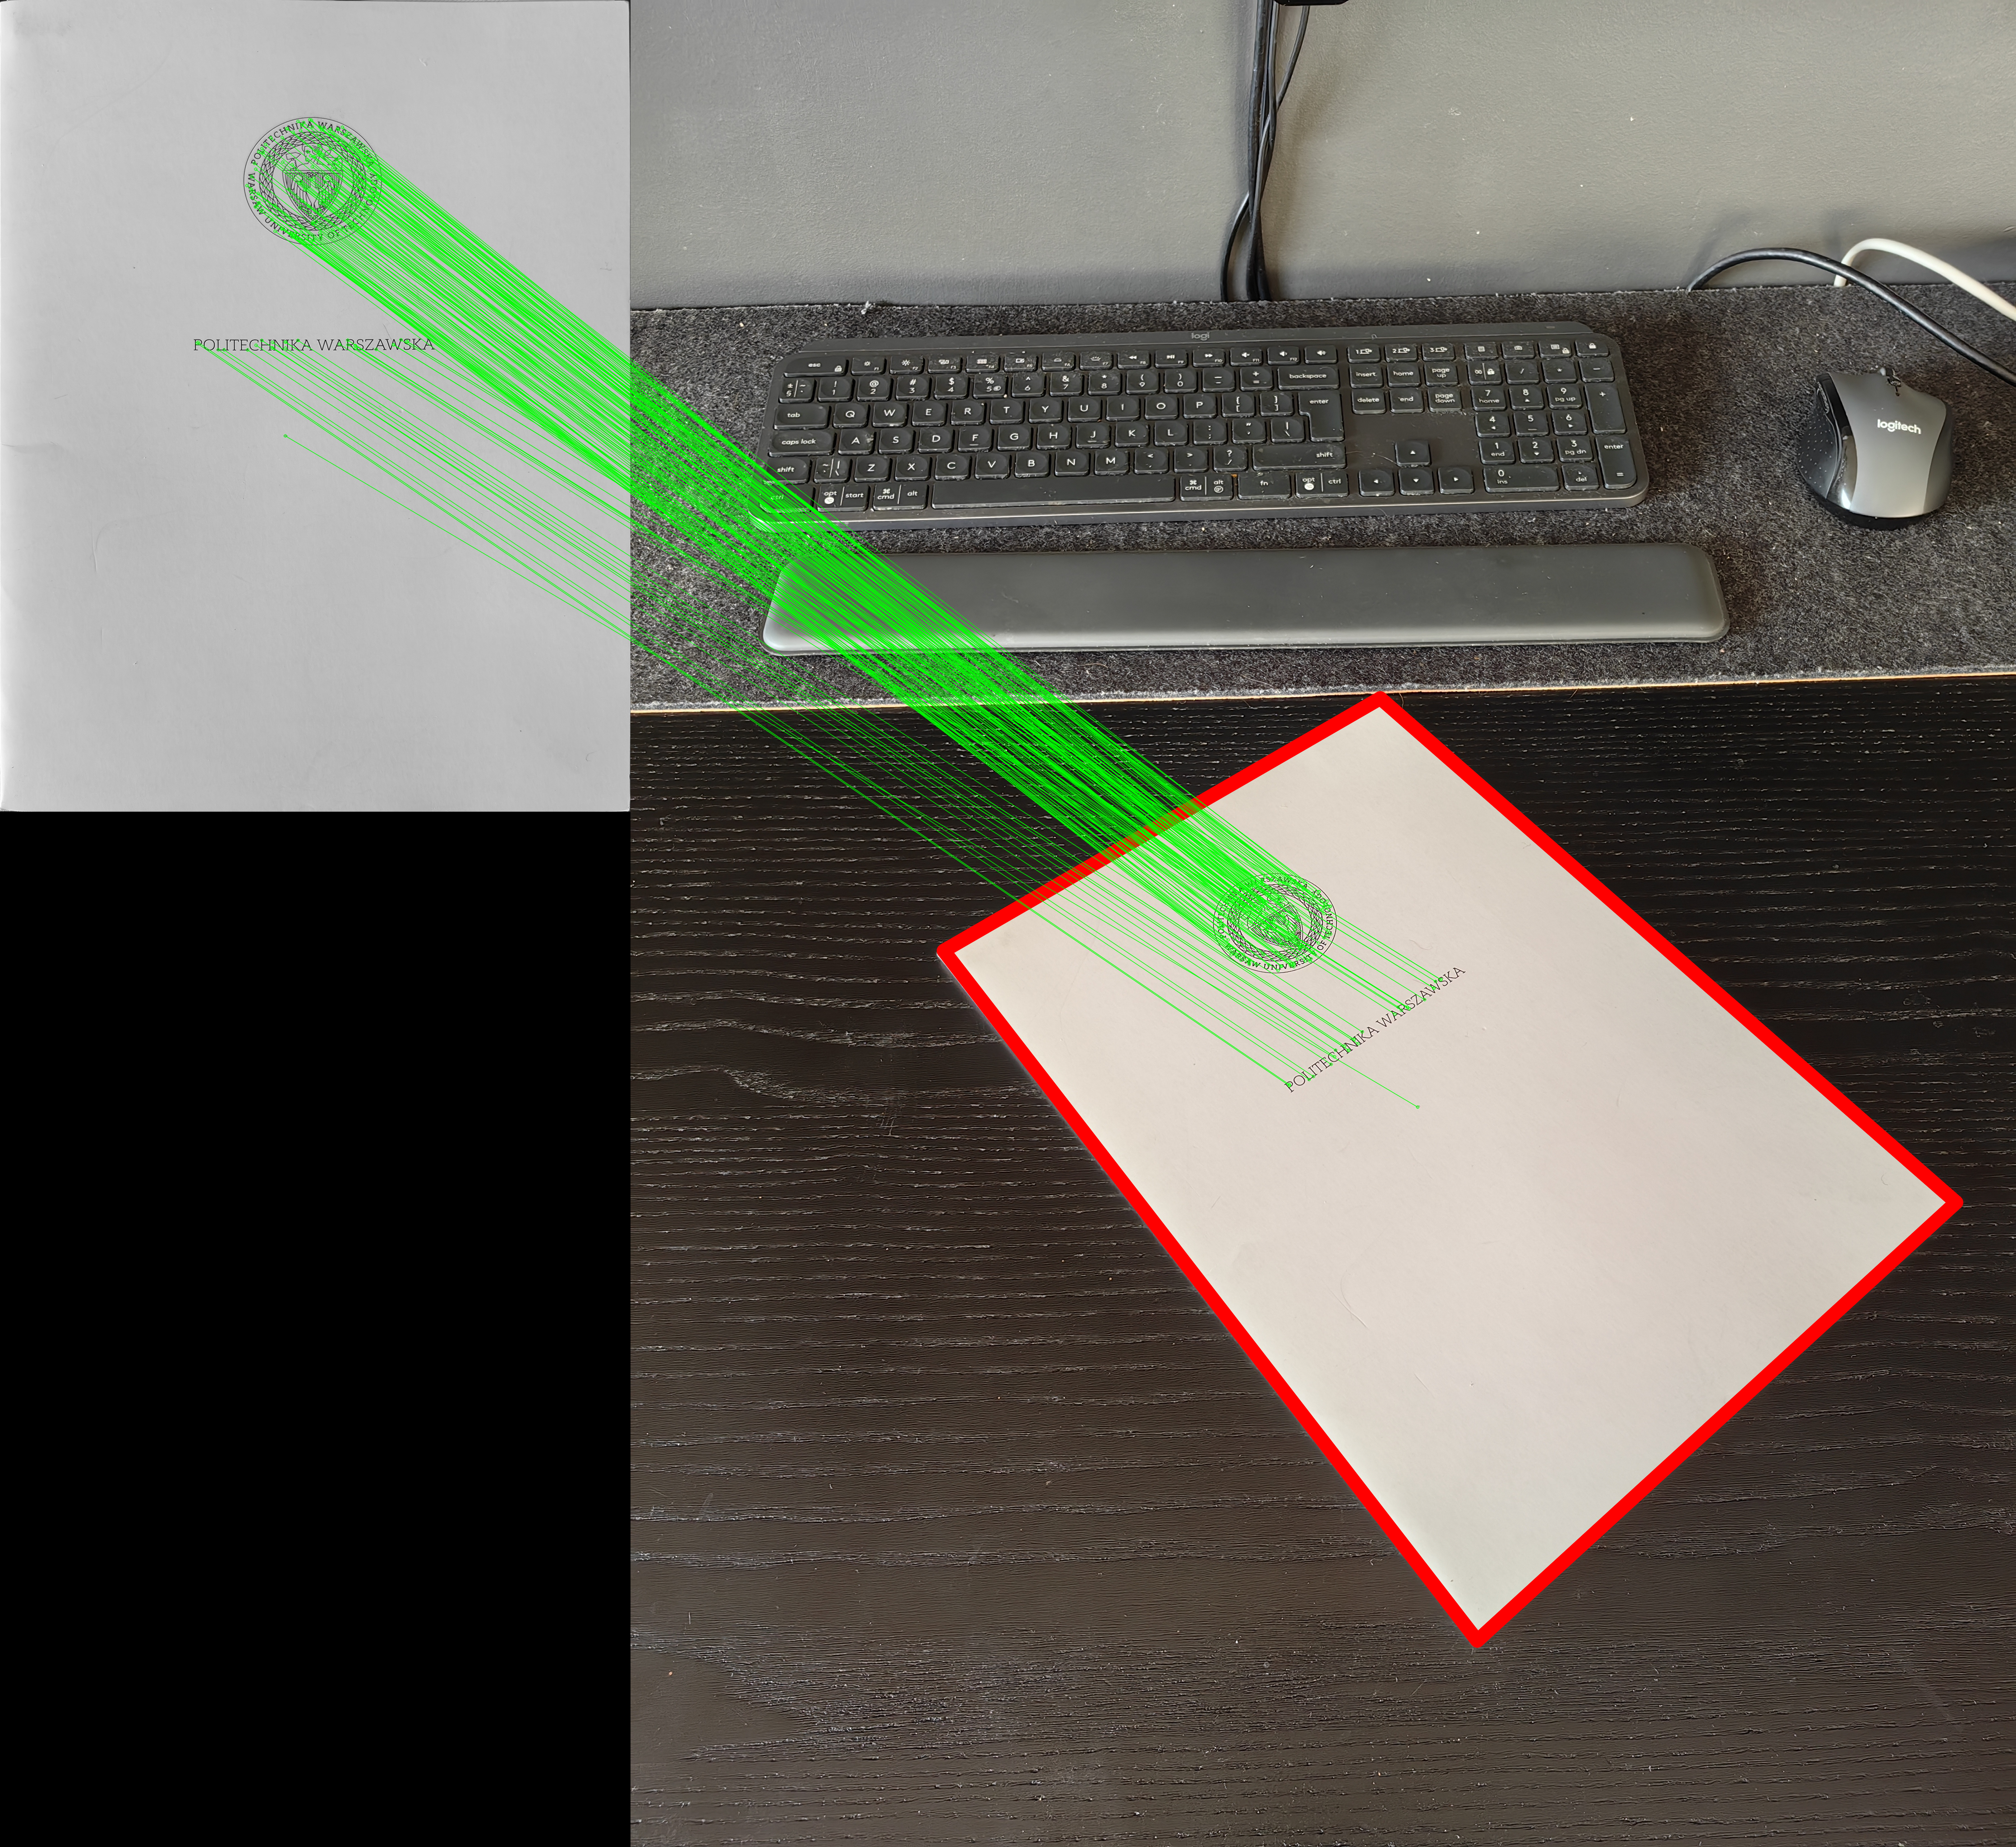
\includegraphics[width=0.65\linewidth]{img/homography.png}
    \caption{Przykład transformacji homograficznej na podstawie dopasowanych punktów kluczowych celem oznaczenia położenia szukanego szablonu.}
    \label{fig:homography}
\end{figure}

W części badawczej pracy dyplomowej do znalezienia optymalnej macierzy homografii wykorzystywane są dwie metody: RANSAC i PROSAC. Mają one za zadanie przeszukiwanie przestrzeni danych oraz obliczenie wartości tej macierzy. 

\paragraph{RANSAC.} Pierwszą z opisywanych metod wykorzystywanych do obliczenia macierzy homografii na podstawie punktów kluczowych jest RANSAC (z ang. Random Sample Consensus) \cite{ransac}. Jest to iteracyjny algorytm służący do estymowania wybranych parametrów na podstawie zestawu danych wejściowych. W przypadku feature matching jest to wyliczenie wartości macierzy transformacji homograficznej, gdy na wejściu zostaje przesłany zestaw punktów kluczowych. Jego celem jest znalezienie jak najlepszego modelu pasującego do jak największej części zbioru.

Algorytm ten według literatury jest skuteczny przy pracy z zaszumionymi danymi oraz ze zbiorami zawierającymi wiele wartości odstających. Wynika to z faktu, że skupia się on na znalezieniu modelu, który pasuje do jak największego zbioru będącego w pewnej odległości od siebie, ignorując przy tym wartości znacznie się różniące i odstające.

W trakcie danej iteracji metody RANSAC wykonywane są następujące kroki:

\begin{enumerate}
    \item Losowy wybór minimalnego zbioru danych potrzebnego do estymowania parametrów. W przypadku dopasowania obrazów zawsze są to co najmniej cztery punkty kluczowe.
    \item Na podstawie wybranego podzbioru obliczane są parametry modelu. W opisywanym kontekście są to wartości macierzy homografii.
    \item Stwierdzenie jaka część danych wykorzystując stworzony model mieści się w granicach ustalonej tolerancji. 
    \item Na podstawie danych będących w ustalanych granicach obliczana jest jakość wygenerowanego modelu. 
\end{enumerate}

Kroki te powtarza się przez określoną liczbę iteracji lub do znalezienia modelu o~wystarczająco wysokim wskaźniku jakości. W pierwszym przypadku wybierany jest ten model ze wszystkich wygenerowanych, dla którego największy podzbiór danych spełnia założone dopasowanie. 


\paragraph{PROSAC.} Kolejnym prezentowanym rozwiązaniem jest PROSAC (ang. Progressive Sample Consensus) \cite{prosac}. Jest to rozwinięcie algorytmu RANSAC poprzez zmianę sposobu wyboru podzbioru danych. W pierwszym z opisywanych podejść jest to wykonywane przez losowy wybór próbek. Natomiast, w przypadku algorytmu PROSAC próbkowanie to odbywa się metodą progresywną na podstawie wyników z poprzednich iteracji. Biorąc pod uwagę oceny ostatnich modeli, priorytezuje on te dane, które są bardziej prawdopodobne. Skupienie się na prawidłowych próbkach ma na celu zwiększenie szansy na szybsze znalezienie dobrego i wystarczającego modelu. Pozostałe kroki są takie same jak w RANSAC. Rozwiązanie to jest częściej wykorzystywane, gdy istnieje duża liczba wartości odstających w zbiorze danych oraz potrzebne jest szybsze dopasowanie modelu. 